En esta sección se detallarán los casos de uso pertenecientes al subsistema de búsqueda. La figura \ref{fig:casos_uso_subsistema_busqueda} muestra el diagrama de casos de uso de dicho subsistema.

\begin{figure}[h]
\centering
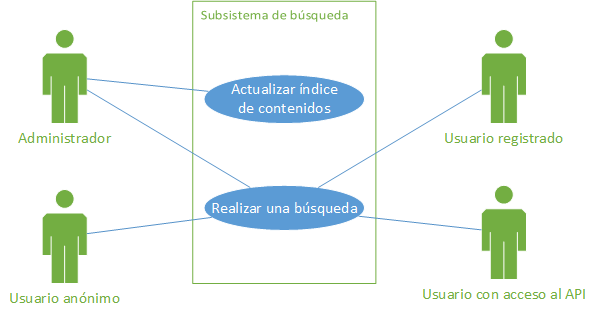
\includegraphics{casos_uso_busqueda}
\caption{Diagrama de casos de uso del subsistema de búsqueda}
\label{fig:casos_uso_subsistema_busqueda}
\end{figure}

\subsubsection{Caso de uso ``realizar una búsqueda''}
\begin{description}
\item[Descripción] Un usuario busca información en el sistema.
\item[Actores] Cualquier rol de usuario.
\item[Escenario principal] \hfill \\	\begin{enumerate}
							\item El usuario introduce un texto en el formulario de búsqueda
							\item El usuario pulsa el botón de buscar
							\item El sistema devuelve los resultados correspondientes
							\end{enumerate}						
\end{description}

\subsubsection{Caso de uso ``actualizar índice de contenidos''}
\begin{description}
\item[Descripción] El administrador actualiza el índice de contenidos del subsistema de búsqueda.
\item[Actores] El administrador del sistema.
\item[Escenario principal] \hfill \\ 	\begin{enumerate}
							\item El administrador accede al panel de control de la búsqueda
							\item El usuario pulsa el botón correspondiente a la opción de regeneración del índice de contenidos.
							\item El sistema actualiza el índice de contenidos incluyendo los nuevos contenidos y eliminado los contenidos que ya no existan.
							\end{enumerate}						
\end{description}